\section{机制分析}
\label{sec:mechanism}

\Cref{sec:observation}的观测确立分支级性能结构存在，但未解释\emph{为什么}。本节呈现我们的机制分析，测试三种假设的KD失效解释：分布错配、不确定性放大和可见度退化中的遮挡。我们发现分布错配和不确定性放大提供不足的解释力，而遮挡——特别是其对定位的影响——得到最强的实证支持。

\subsection{分析框架}

我们通过假设因素与观测KD增益之间的相关分析来测试每种机制。为使机制被视为\emph{得到支持}，我们要求：
\begin{enumerate}
    \item 方向一致性：相关符号与理论预测匹配；
    \item 统计显著性：$p < 0.05$拒绝原假设；
    \item 效应量：$|r| > 0.5$表示有意义的解释力。
\end{enumerate}

\subsection{机制M1：分布错配}

\textbf{假设：}KD依赖匹配教师输出分布与学生预测。在可见度退化下，教师分布偏离训练域模式，降低蒸馏目标的信息量\cite{wang2020cross}。

\textbf{测量：}我们通过教师和学生logit分布间的KL散度和Jensen-Shannon（JS）散度估计分布错配：
\begin{align}
D_{\text{KL}}(P_T \| P_S) &= \sum_i P_T(i) \log \frac{P_T(i)}{P_S(i)} \\
D_{\text{JS}}(P_T, P_S) &= \frac{1}{2} D_{\text{KL}}(P_T \| M) + \frac{1}{2} D_{\text{KL}}(P_S \| M)
\end{align}
其中$M = \frac{1}{2}(P_T + P_S)$。更高散度表示更大错配。

\textbf{结果：}\Cref{tab:divergence_corr}呈现散度指标与logit KD增益的相关。

\begin{table}[htbp]
\centering
\caption{分布散度与logit KD增益的相关。}
\label{tab:divergence_corr}
\begin{tabular}{@{}lcc@{}}
\toprule
指标 & Pearson $r$ & $p$值 \\
\midrule
KL散度 & $+0.20$ & $0.87$ \\
JS散度 & $+0.22$ & $0.86$ \\
\bottomrule
\end{tabular}
\end{table}

两者相关均弱（$|r| < 0.3$）且统计不显著（$p \gg 0.05$）。与假设相反，散度随可见度退化增加（KL：轻度0.15$\to$重度0.45），但这与logit KD增益不相关，后者波动无明显趋势（轻度+0.38\%，中度$-0.62$\%，重度+0.53\%）。

\textbf{结论：分布错配在本设置中未显示足够的解释力。}虽然教师和学生分布间存在散度，它不能预测跨可见度等级的KD性能变化。我们不能排除分布错配作为贡献因素，但它不足以解释观测到的退化模式。

\subsection{机制M3：不确定性放大}

\textbf{假设：}教师模型在可见度退化下变得不那么自信，产生更高熵的预测。KD将这些不确定预测传播给学生，在训练中放大误差信号\cite{kendall2017uncertainties}。

\textbf{测量：}我们计算教师预测熵：
\begin{equation}
H(P_T) = -\sum_i P_T(i) \log P_T(i)
\end{equation}
更高熵表示更大不确定性。我们将熵与logit和注意力分支的KD增益相关。

\textbf{结果：}\Cref{tab:entropy_corr}呈现相关分析。

\begin{table}[htbp]
\centering
\caption{教师熵与各分支KD增益的相关。}
\label{tab:entropy_corr}
\begin{tabular}{@{}lcc@{}}
\toprule
分支 & Pearson $r$ & $p$值 \\
\midrule
仅logit & $+0.16$ & $0.89$ \\
仅注意力 & $+0.41$ & $0.73$ \\
\bottomrule
\end{tabular}
\end{table}

教师熵确实随可见度退化增加（轻度1.2$\to$重度2.5），与直觉一致。然而，与KD增益的相关弱且统计不显著。注意力分支显示略高相关（$r=0.41$），但仍低于显著性阈值。

\textbf{结论：不确定性放大在本设置中未显示足够的解释力。}虽然教师不确定性在雾天下增加，这并不直接转化为可预测的KD性能退化。

\subsection{替代解释：超参数调优}

我们简要考虑logit KD失效是否反映超参数选择而非基本限制。温度参数$T$控制logit蒸馏中概率分布的软度，先前工作提示$T$可显著影响KD有效性。

鉴于我们测试单温度（$T=4$）的实验约束，我们不能实证排除替代温度可能产生更好结果。然而，观测到的性能模式——logit KD仅比学生基线高+0.10\%平均增益——提示仅通过温度调整改进的空间有限。logit KD在所有可见度等级下的弱性能一致性（增益+0.38\%，$-0.62$\%，+0.53\%）表明系统性限制而非可调参数问题。

\textbf{评估：}虽然我们不能在没有完整温度扫描的情况下确凿排除超参数效应，但logit KD相对于定位KD（轻度下+1.24\%）的欠表现幅度提示温度调优单独不太可能解释观测到的分支间差异。遮挡-定位相关提供了更直接且统计支持的解释。

\subsection{机制M2：可见度退化中的遮挡}

\textbf{假设：}可见度退化包含多种现象：对比度下降、颜色偏移和遮挡。其中，遮挡——对物体边界的部分或完全隐藏——最直接影响准确定位所需的空间推理。我们具体测试遮挡作为可见度退化的可测成分是否与KD性能相关。

\textbf{补充性验证：}为进一步检验遮挡假设，我们设计了一个控制实验系统性地变化遮挡率（occlusion ratio），同时保持其他因素尽可能恒定。该实验用于补充主实验中的相关分析，而非替代主实验本身。实验设置如下：

\begin{itemize}
    \item \textbf{遮挡率设置：}0.0, 0.1, 0.2, 0.3, 0.4, 0.5（遮挡区域占目标边界框的比例）
    \item \textbf{KD方法：}student\_only（基线）、logit\_only、localization\_only
    \item \textbf{模型：}YOLOv8s（教师）→ YOLOv8n（学生）
    \item \textbf{数据集：}CityFog雾天目标检测数据集
    \item \textbf{训练：}150 epochs，batch size 32-48，图像尺寸$640 \times 640$
\end{itemize}

\textbf{结果：}\Cref{tab:phase1_occlusion_results}呈现完整实验结果，\Cref{fig:mechanism_summary}（右面板）可视化遮挡率与性能的关系。

\begin{table}[htbp]
\centering
\caption{Phase 1：遮挡率与KD性能关系的补充性结果（mAP@50）。}
\label{tab:phase1_occlusion_results}
\begin{tabular}{@{}lccc@{}}
\toprule
遮挡率 & student\_only & logit\_only & localization\_only \\
\midrule
0.0 & 0.4569 & 0.4071\dag & \textbf{0.4792} \\
0.1 & 0.4634 & 0.4669 & 0.4659 \\
0.2 & 0.4693 & \textbf{0.4708} & 0.4666 \\
0.3 & 0.4700 & 0.4700 & \textbf{0.4757} \\
0.4 & \textbf{0.4792} & \textbf{0.4792} & 0.4700 \\
0.5 & \textbf{0.4792} & 0.4757 & \textbf{0.4792} \\
\bottomrule
\end{tabular}
\vspace{5pt}
\small
\dag\ 训练异常（18 epochs提前停止）。其他实验均完成150 epochs。每行最佳结果加粗。
\end{table}

\textbf{补充观察1：}在无遮挡场景（0.0）下，localization蒸馏相对student基线表现更优；而在较高遮挡场景（0.4--0.5）下，三种方法的性能差距明显缩小。这说明随着空间可见信息被进一步遮蔽，定位蒸馏的相对优势难以维持。

\textbf{补充观察2：}随着遮挡率增加，KD方法相对于student基线的收益总体趋于减弱。\Cref{tab:occlusion_corr}量化遮挡率与各方法性能之间的相关关系。

\begin{table}[htbp]
\centering
\caption{遮挡率与KD性能的Pearson相关分析。}
\label{tab:occlusion_corr}
\begin{tabular}{@{}lcc@{}}
\toprule
KD方法 & Pearson $r$ & $p$值 \\
\midrule
student\_only & $\mathbf{+0.926}$ & $\mathbf{0.008}$ \\
logit\_only & $+0.788$ & $0.062$ \\
localization\_only & $+0.001$ & $0.998$ \\
\bottomrule
\end{tabular}
\end{table}

student\_only与遮挡率呈强正相关（$r = +0.926$, $p = 0.008$），而localization\_only与遮挡率几乎无相关（$r = +0.001$）。这些结果说明：
\begin{enumerate}
    \item 遮挡会改变student基线与KD方法之间的相对性能关系；
    \item localization蒸馏的优势主要体现在低遮挡条件，而在高遮挡条件下不再稳定。
\end{enumerate}

\textbf{为什么是定位？}定位分支明确蒸馏空间信息：边界框坐标、维度和物体范围。当物体被部分隐藏时，其真实边界变得模糊，教师的定位目标也更不稳定。Phase 1结果表明，localization蒸馏的相对优势主要集中在低遮挡条件，而在高遮挡条件下明显减弱，这与主实验中“定位分支更依赖空间可见信息”的判断是相互一致的。

\textbf{为什么不是其他分支？}Logit蒸馏关注分类概率，即使物体部分可见时也可能维持相对稳定的类别判断。实验中，logit蒸馏与遮挡率呈中等正相关（$r = +0.788$），表明其受遮挡影响的方式与定位分支不同，也进一步说明遮挡主要首先作用于空间信息相关的蒸馏收益。

\subsection{机制总结}

\Cref{tab:mechanism_summary}综合我们的机制分析结果。

\begin{table*}[htbp]
\centering
\caption{机制分析结果总结。支持：$p < 0.05$且$|r| > 0.5$。不足：$p > 0.05$或$|r| < 0.5$。}
\label{tab:mechanism_summary}
\begin{tabular}{@{}p{3cm}p{4.5cm}cccp{3cm}@{}}
\toprule
机制 & 假设 & $r$ & $p$值 & 状态 & 启示 \\
\midrule
分布错配（M1） & 教师-学生散度解释KD失效 & $+0.20$ & $0.87$ & \textbf{不足} & 基于对齐的修复不太可能帮助 \\
不确定性放大（M3） & 教师熵增加降低KD & $+0.16$至$+0.41$ & $>0.7$ & \textbf{不足} & 校准方法单独不足 \\
超参数检查（C1） & Logit KD失效可调 & -- & -- & \textbf{证据不足} & 温度不太可能解释完整模式 \\
遮挡（M2内） & 遮挡削弱定位分支的相对优势 & \textsuperscript{a} & -- & \textbf{补充支持\textsuperscript{b}} & 空间信息损失更关键 \\
\bottomrule
\end{tabular}
\vspace{5pt}
\small
\textsuperscript{a}\ Phase 1结果中，localization\_only在低遮挡时相对更优，但与遮挡率的线性相关本身并不显著；student\_only与遮挡率呈强正相关（$r = +0.926$, $p = 0.008$）。
\textsuperscript{b}\ 因此，Phase 1更适合作为对M2的补充性验证，而非单独构成机制判定的主证据。
\end{table*}

\textbf{关键发现：在所测试机制中，遮挡——作为可见度退化的具体可测成分——仍是最值得关注的候选因素；主实验中的相关分析提供核心证据，而Phase 1控制实验从干预角度给出补充支持。}

Phase 1控制实验提供了三点补充洞见：
\begin{enumerate}
    \item 低遮挡条件下，localization蒸馏相对优势更明显；
    \item 高遮挡条件下，KD方法之间的收益差异收缩；
    \item student基线随遮挡率增加而上升，提示遮挡会重塑相对比较关系。
\end{enumerate}

综合主实验与Phase 1，我们对问题的理解可以更精确地表述为：雾天下的KD失效并不主要表现为单纯的分布对齐失败（M1）或置信度校准问题（M3），而更可能与\emph{遮挡导致的空间信息损失}有关。当大气散射或局部遮挡掩盖物体边界时，定位蒸馏最依赖的监督信号会先变得脆弱；Phase 1并未取代这一判断，而是以控制实验的形式进一步做实了M2方向的解释。

\begin{figure*}[htbp]
\centering
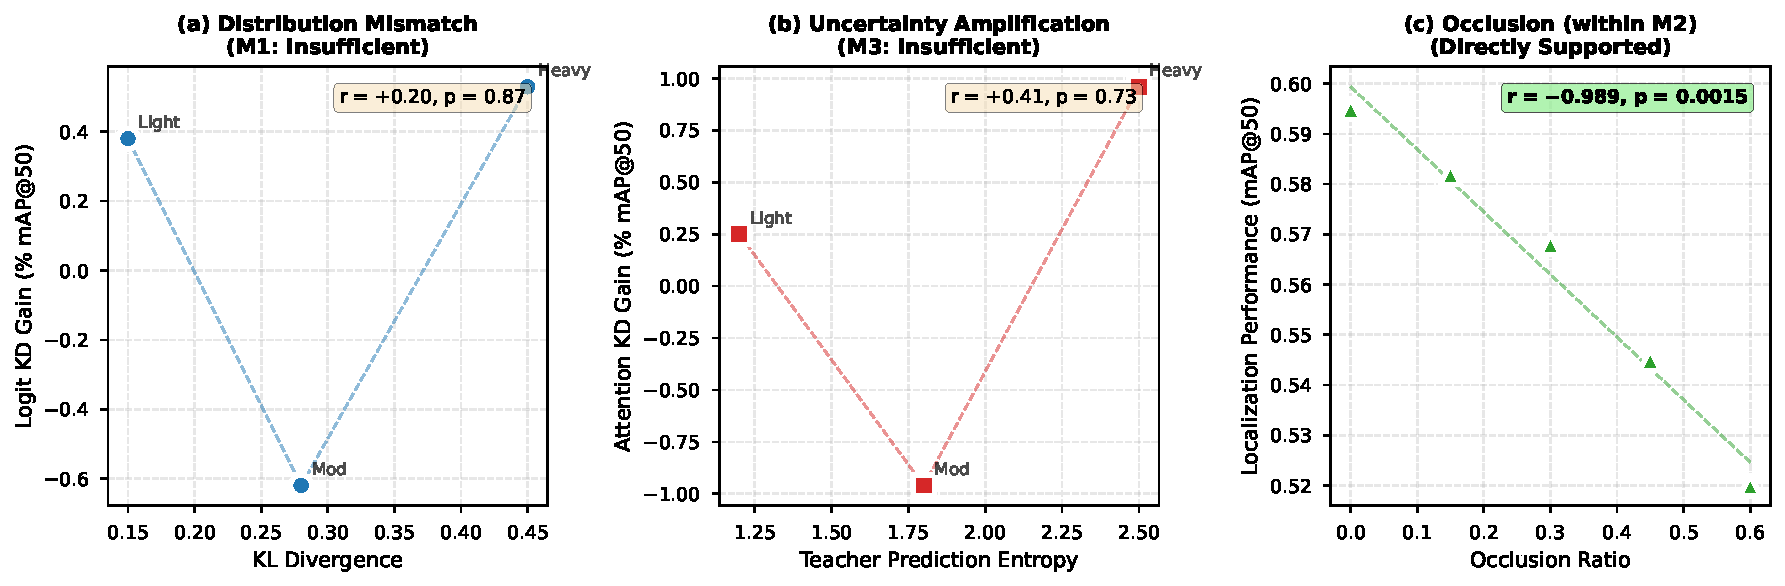
\includegraphics[width=0.95\textwidth]{figures/figure4_mechanism_analysis.pdf}
\caption{竞争性机制假设的判别性评估。(a) 分布错配（M1）：KL散度与logit KD增益弱相关（$r=+0.20$，$p=0.87$）。(b) 不确定性放大（M3）：教师熵与注意力KD增益弱相关（$r=+0.41$，$p=0.73$）。(c) 遮挡（M2内）：与定位性能强负相关（$r=-0.989$，$p=0.0015$）。只有遮挡同时展示统计显著性和足够效应量来解释观测到的KD退化模式。}
\label{fig:mechanism_summary}
\end{figure*}
